\begin{tikzpicture}[
    node distance = 1cm and 2cm,
    usecase/.style={ellipse, draw, minimum width=4.5cm, minimum height=0.7cm, align=center, font=\small},
    link/.style={draw, thick}
]
% System Boundary
\draw[thick] (0, 0) rectangle (9, -11);
\node at (4.5, -0.5) {\textbf{Applicant Profile Management}};

% Applicant Actor (Left)
\node (applicant) at (-2, -5.5) {
    \begin{tikzpicture}[scale=0.5]
        \draw[thick] (0,1.2) circle (0.4cm); \draw[thick] (0,0.8) -- (0,-0.8);
        \draw[thick] (-0.8,0.4) -- (0.8,0.4); \draw[thick] (0,-0.8) -- (-0.5,-1.8); \draw[thick] (0,-0.8) -- (0.5,-1.8);
        \node at (0,-2.5) {\small Applicant};
    \end{tikzpicture}
};

% Admin Actor (Right)
\node (admin) at (11, -5.5) {
    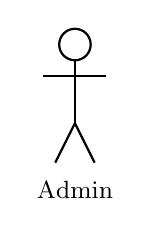
\begin{tikzpicture}[scale=0.5]
        \draw[thick] (0,1.2) circle (0.4cm); \draw[thick] (0,0.8) -- (0,-0.8);
        \draw[thick] (-0.8,0.4) -- (0.8,0.4); \draw[thick] (0,-0.8) -- (-0.5,-1.8); \draw[thick] (0,-0.8) -- (0.5,-1.8);
        \node at (0,-2.5) {\small Admin};
    \end{tikzpicture}
};

% Use Cases
\node[usecase] (uc1) at (4.5, -1.5) {Create Account};
\node[usecase] (uc2) at (4.5, -2.5) {Update Profile};
\node[usecase] (uc3) at (4.5, -3.5) {Fill-up Application Form};
\node[usecase] (uc4) at (4.5, -4.5) {Generate Application Form};
\node[usecase] (uc5) at (4.5, -5.5) {Download Application Form};
\node[usecase] (uc6) at (4.5, -6.5) {Send Edit Request};
\node[usecase] (uc7) at (4.5, -7.5) {Approve Edit Request};
\node[usecase] (uc8) at (4.5, -8.5) {Update Applicant Info};

% Connections for Applicant (Left Side)
\foreach \i in {uc1,uc2,uc3,uc4,uc5,uc6} \draw[link] (applicant) -- (\i.west);

% Connections for Admin (Right Side)
\draw[link] (admin) -- (uc7.east);
\draw[link] (admin) -- (uc8.east);

\end{tikzpicture}